\documentclass{standalone}
\usepackage{tikz}
\usepackage{pxfonts}

\usetikzlibrary{shadows, calc}

\begin{document}

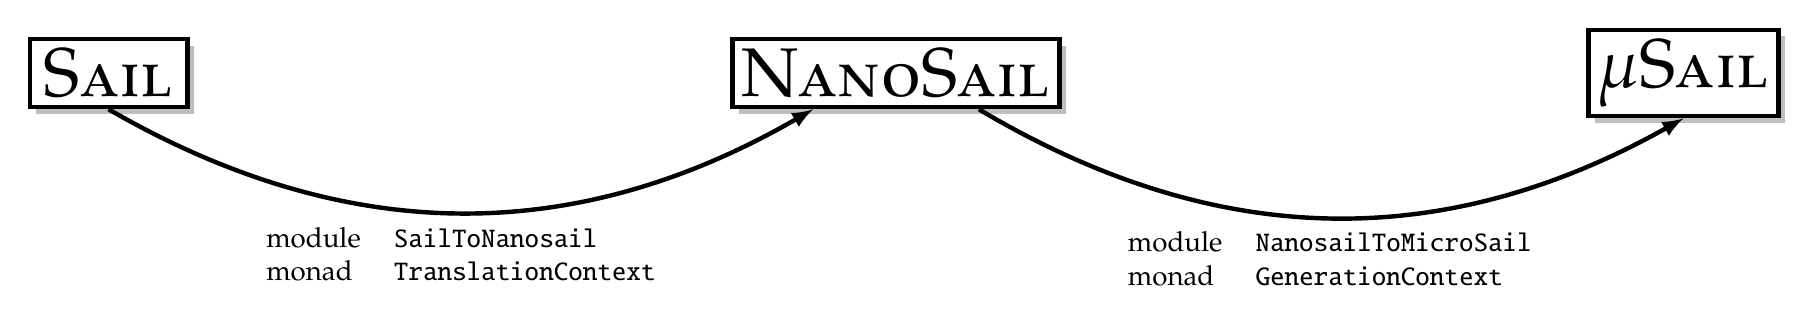
\begin{tikzpicture}[language/.style={minimum width=2cm,minimum height=8mm,draw,fill=white,drop shadow,font=\sc\Huge,ultra thick},
                    translation arrow/.style={-latex, ultra thick}]
  \node[language] (sail) at (0, 0) {Sail};
  \node[language] (nanosail) at (10, 0) {NanoSail};
  \node[language] (microsail) at (20, 0) {$\mu$Sail};

  \path[translation arrow] (sail.south) edge[bend right=30] node[below, midway] {
    \begin{tabular}{ll}
      module & \texttt{SailToNanosail} \\
      monad & \texttt{TranslationContext} \\
    \end{tabular}
  } ($ (nanosail.south west) ! 0.5 ! (nanosail.south) $);
  
  \path[translation arrow] ($ (nanosail.south) ! 0.5 ! (nanosail.south east) $) edge[bend right=30] node[below,midway] {
    \begin{tabular}{ll}
      module & \texttt{NanosailToMicroSail} \\
      monad & \texttt{GenerationContext} \\
    \end{tabular}
  } (microsail.south);
\end{tikzpicture}

\end{document}